\chapter{Classification results evaluation} \label{chapt4}

\section{General steps} \label{sect4_1}
\noindent
In this section I need to:
\begin{itemize}
	\item visualize results of each training step, to understand hyperparameters better
	\item estimate networks by types 
	\item chose hyperparameters to gain the best evaluation metrics  
	\item train each network on different amount of epochs
	\item save network parameters and weights after each epoch. It will give me a possibility it will be easy to restore the best model if network accuracy will go down.
\end{itemize}

\noindent
Training time is very important parameter. Therefore, I would like train NN models which have nearly the same training time. To make it easier to understand results of NN, the famous suite of visualization tools called TensorBoard was used. With TensorBoard it is possible to visualize graphs, plot quantitative metrics and show additional data like images that pass through it.  


\section{Base line model} \label{sect4_2}

Firstly, I built the baseline model which CNN models should achieve in the future. I started this step with LSTM networks, as most often mentioned in articles with NLP problems. On this step I was trying different configurations of LSTM parameters. The architecture which gave me the best score is shown in the Figire \ref{img:part4-bilstm}. According to my experiments bidirectional recurrent networks perform better than the same type and same size by parameters one directional networks, therefore it was chosen as the main layer. As input to the NN I give two embedded sequences of words: one for the description of advert , another for title. This model has the bi-LSTM layer with 100 units. Each sequence go through the bi-LSTM layer and then merged together. To solve overfitting in this model I used BatchNormalization and dropout. LSTM dropout rate was chosen manually and was equal to 0.332. Besides the bi-LSTM layer, there are two fully connected layers: one at the end because we want to estimate probabilities for each class, so it has 183 neurons in it and one in the middle with 130 neurons. As a training algorithm I chose Adam with default parameters: (lr=0.001, beta\_1=0.9, beta\_2=0.999, epsilon=1e-08, decay=0.0). As I have mentioned earlier, for better understanding of the network I visualize the histograms and percentile weights in each layer. The model was trained on 15 epochs.


\begin{figure}[ht] 
	\center
	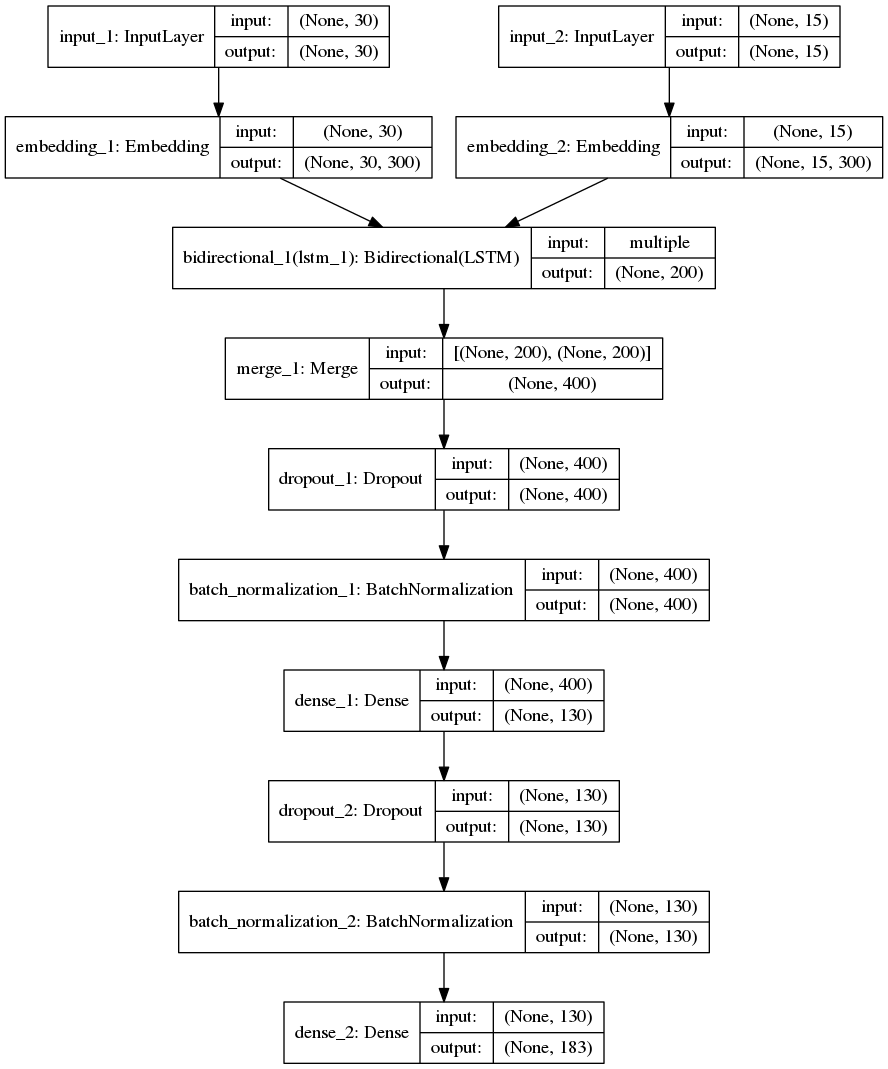
\includegraphics [scale=0.4] {part4/bilstm_architecture.png}
	\label{img:part4-bilstm}  
	\caption{Architectures of Bi-LSTM models with 100 units } 
\end{figure}

As can be seen from the results of model training in the \ref{img:/bilstm_val_category_accuracy}, categorical accuracy on the training set and validation set performs equally good: 0.7975 and 0.8203 respectively. Surprisingly, results on train are slightly better than on training data.   

\begin{figure}[ht]
	\begin{minipage}[ht]{1\linewidth}
		\center{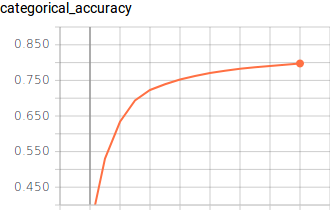
\includegraphics[width=0.5\linewidth]{part4/bilstm_train_category_accuracy}}
	\end{minipage}
	\hfill
	\begin{minipage}[ht]{1\linewidth}
		\center{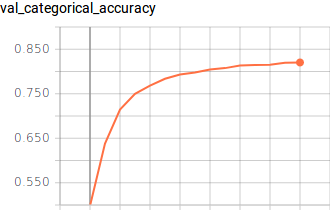
\includegraphics[width=0.5\linewidth]{part4/bilstm_val_category_accuracy}}
	\end{minipage}
	\caption{Models train and validation categorical accuracy by epochs}
	\label{img:/bilstm_val_category_accuracy}  
\end{figure}

Figure \ref{img:bilstm_val_category_crossentropy} shows that categorical cross entropy decrease on each epoch as it was expected. After 15 epochs results were following: 0.8532 on the training set and 0.7478 on test.    

\begin{figure}[ht]
	\begin{minipage}[ht]{1\linewidth}
		\center{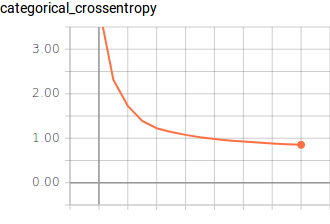
\includegraphics[width=0.5\linewidth]{part4/bilstm_train_category_crossentropy}}
	\end{minipage}
	\hfill
	\begin{minipage}[ht]{1\linewidth}
		\center{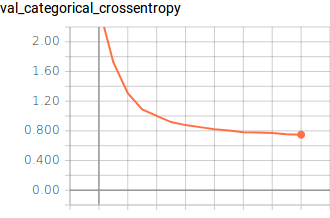
\includegraphics[width=0.5\linewidth]{part4/bilstm_val_category_crossentropy}}
	\end{minipage}
	\caption{Models train and validation category crossentropy by epochs}
	\label{img:bilstm_val_category_crossentropy}  
\end{figure}

The most important metric for this task was top categorical accuracy which can be seen in the Figure \ref{img:bilstm_val_top_k_accuracy}. On training data the model showed 0.9189 accuracy and on the test data - 0.9319.   

\begin{figure}[ht]
	\begin{minipage}[ht]{1\linewidth}
		\center{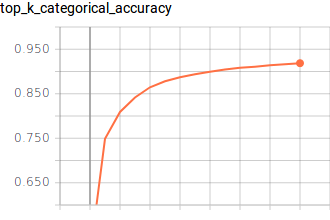
\includegraphics[width=0.5\linewidth]{part4/bilstm_train_top_k_accuracy}}
	\end{minipage}
	\hfill
	\begin{minipage}[ht]{1\linewidth}
		\center{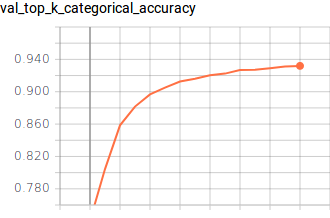
\includegraphics[width=0.5\linewidth]{part4/bilstm_val_top_k_accuracy}}
	\end{minipage}
	\caption{Models train and validation top k accuracy by epochs}
	\label{img:bilstm_val_top_k_accuracy}  
\end{figure}

Additional metrics which interested me in these experiments was time per epoch. These results can be seen in the Figure \ref{img:bilstm_timing}.

\clearpage
\begin{figure}[ht] 
	\center
	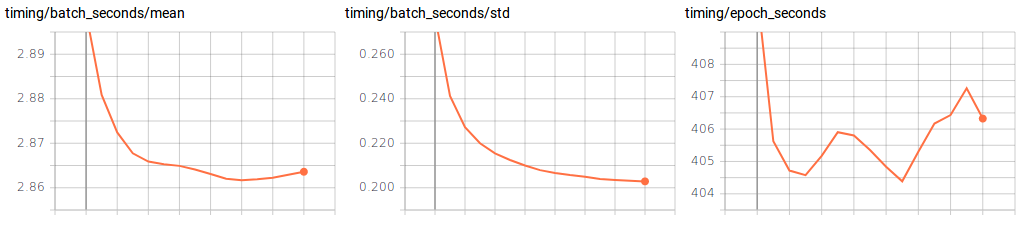
\includegraphics [scale=0.5] {part4/bilstm_timing}
	\caption{Models batch time by epochs} 
	\label{img:bilstm_timing}  
\end{figure}


Histograms give a lot of information about what is happening with the network. I decided to pay attention on histograms which were output from recurrent network - that show bi-LSTM behavior and weights for first layer of feedforward network. I did not find descriptive explanation for how to interpret these kind of graphics, so I followed basic knowledge from statistics. 

\begin{figure}[ht]
	\begin{minipage}[ht]{1\linewidth}
		\center{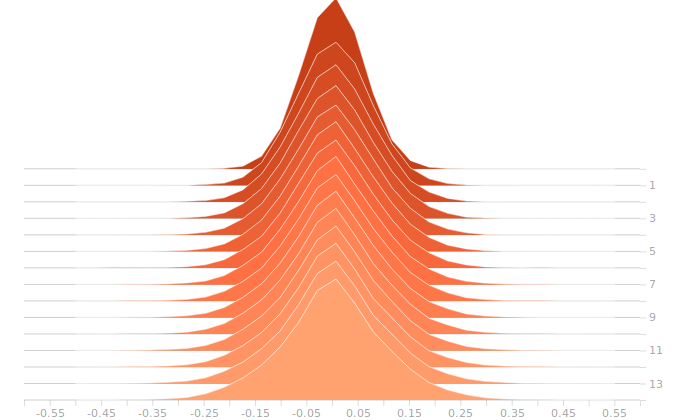
\includegraphics[width=0.5\linewidth]{part4/bilstm_forward_lstm_1_recurrent_kernel_0} \\ а}
	\end{minipage}
	\hfill
	\begin{minipage}[ht]{1\linewidth}
		\center{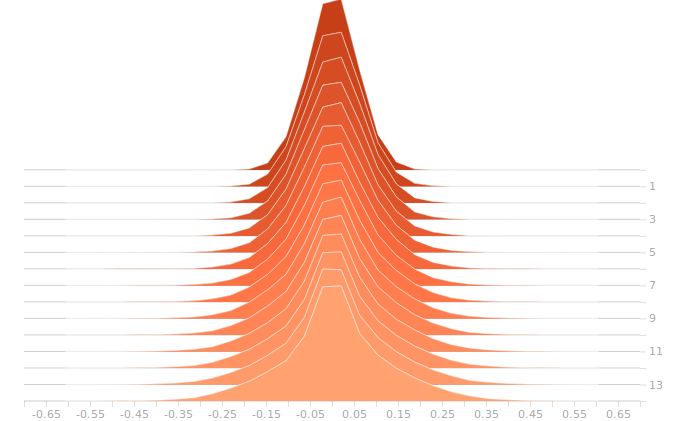
\includegraphics[width=0.5\linewidth]{part4/bilstm_backward_lstm_1_recurrent_kernel_0} \\ b}
	\end{minipage}
	\caption{Bi-LSTM 100 units. Histogram of output from forward recurrent layers (a); histogram of weights from backward recurrent layers (b)}
	\label{img:category_crossentropy}  
\end{figure}


According to the Figures \ref{img:/bilstm_val_category_accuracy}, \ref{img:bilstm_val_category_crossentropy}, \ref{img:bilstm_val_top_k_accuracy} model was not overfitted. Histograms of outputs from feed forward and backward recurrent layers do not change significantly during training process. 
I can interpret this in the way that this layer do not train enough and I think that this network continues to learn thanks to FFNN part. I think, that the best shape for the histogram of weights from first FFNN layer will be normal distribution with higher variance, than after initialization. As we can see the FFNN layer has exactly this behavior which means that it learns some meaningful information. It is possible that more epochs will have a positive affect on the recurrent layer. 

\begin{figure}[ht] 
	\center
	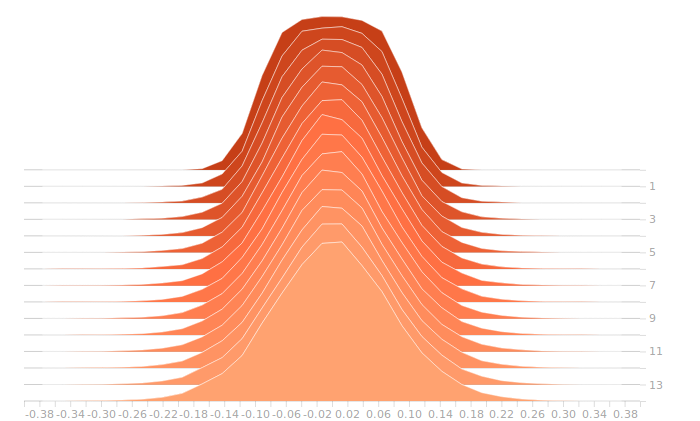
\includegraphics [scale=0.5] {part4/bilstm_dense}
	\caption{Bi-LSTM 100 units. Histogram of weights from first FFNN layer.} 
	\label{img:bilstm_dense}  
\end{figure}

The bi-LSTM model requires a significant amount of computational resources: specially RAM memory.
Therefore, the batch size was chosen equal to 3048. We can see consumption of resources in the Figure \ref{img:resources_BILSTM}


\begin{figure}[ht] 
	\center
	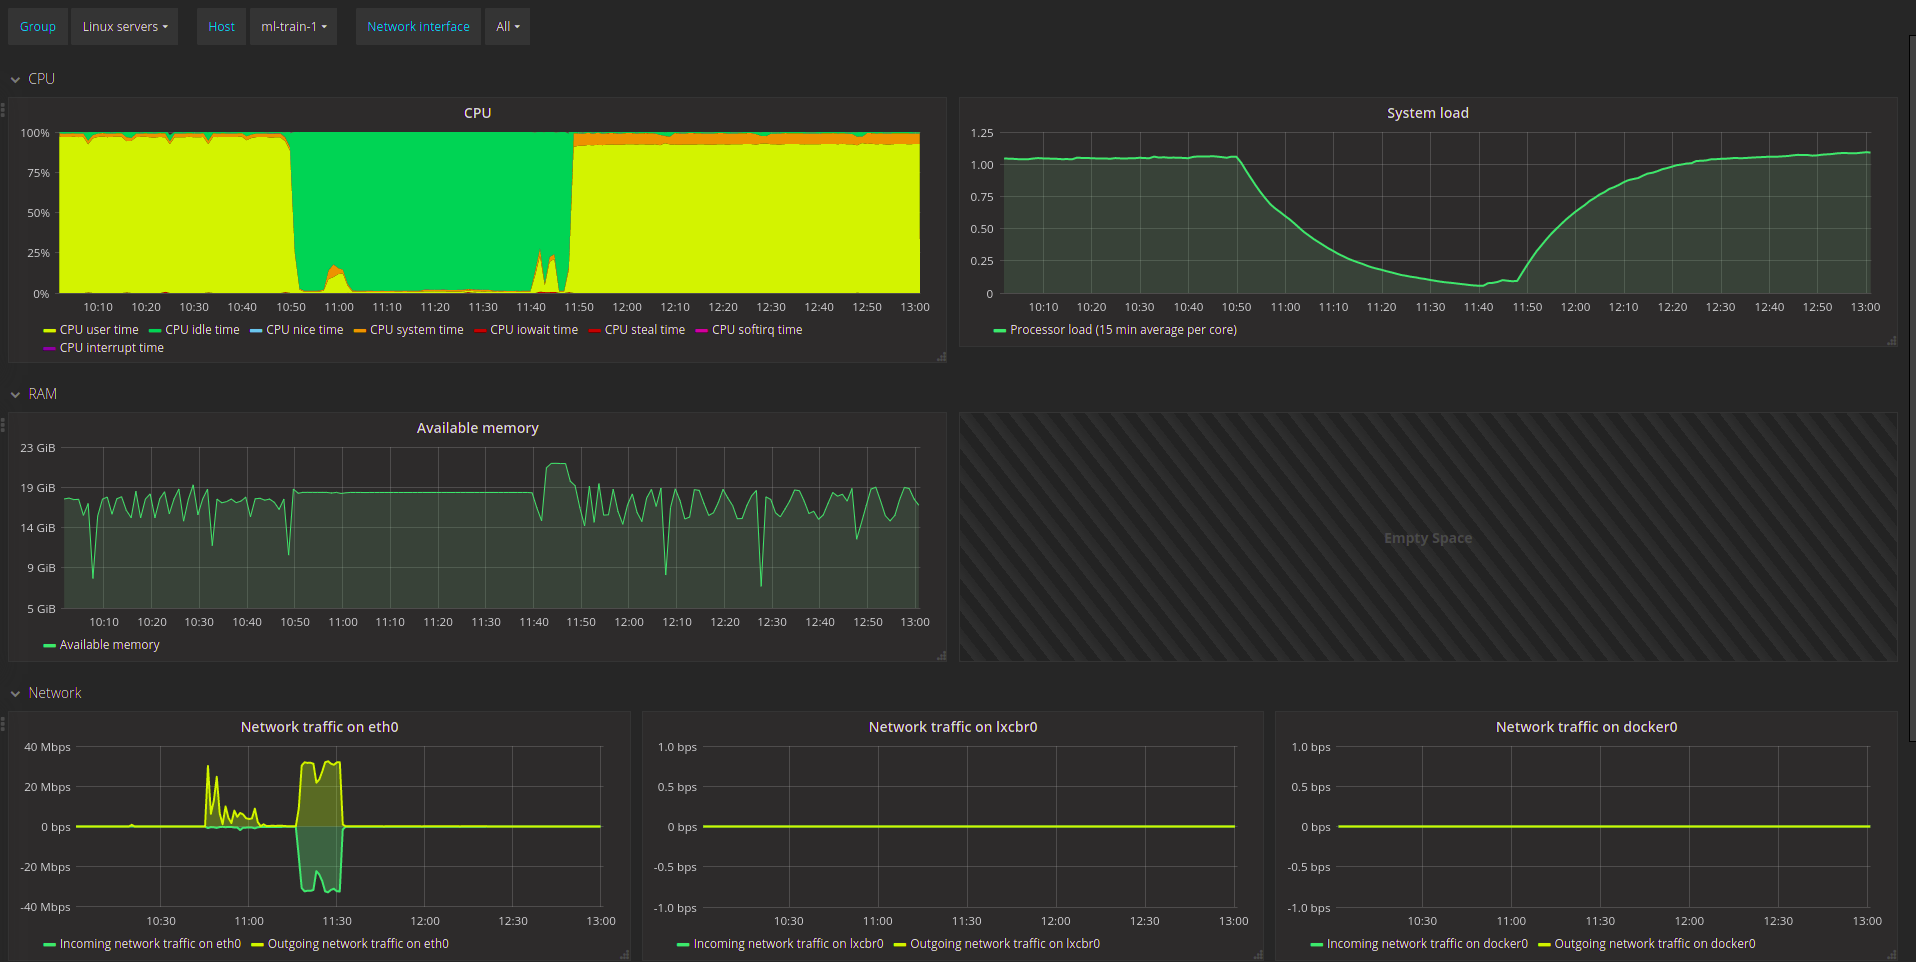
\includegraphics [scale=0.2] {part4/resources_BILSTM}
	\caption{CPU resources which were used while training Bi-LSTM NN.} 
	\label{img:resources_BILSTM}  
\end{figure}


\clearpage
\section{Convolution neural network} \label{sect4_3}

In this part I would like to show that CNN can perform not worst than recurrent based neural networks. Therefore, I implemented CNN architecture Figure \ref{img:cnn_architecture} which was described in the section \ref{sect2_2_1}. I build three model with different numbers of filters. The smallest one contains 128 filter, middle one - 256 and the biggest - 512. All models were trained with the same number of filter: 3, 4, 5 and dropout rate equals to 0.5. I did not use regularization for convolution layers, but according to my experience big pooling window also prevent overfittng.Models were trained on 15 epochs.

Let us compare results which different models give. 

\begin{table}[h]
	\centering
	\caption{Analysis of categorical accuracy}
	\label{my-label}
	\begin{tabular}{| p{7cm} | p{3cm} | p{3cm} |}
		%	\begin{tabulary}{1.0\textwidth}{|L|L|L|L|L|L}
		\hline
		\textbf{Number of filters}  & \textbf{Train} & \textbf{Test}                                                    
		\\ \hline
		128   &  0.8165 & 0.8126
		\\ \hline
		256   &  0.8532 & 0.8251 
		\\ \hline
		512   &  0.8885 & 0.8338
		\\ \hline		
	\end{tabular}
\end{table}


\begin{figure}[ht]
	\begin{minipage}[ht]{1\linewidth}
		\center{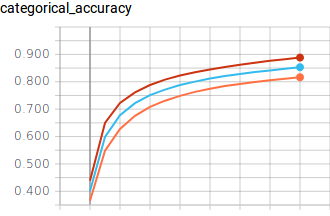
\includegraphics[width=0.5\linewidth]{part4/3CNN_train_category_accuracy}}
	\end{minipage}
	\hfill
	\begin{minipage}[ht]{1\linewidth}
		\center{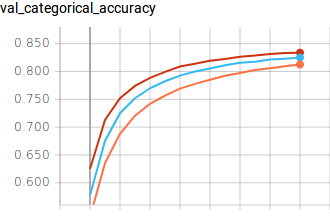
\includegraphics[width=0.5\linewidth]{part4/3CNN_val_category_accuracy}}
	\end{minipage}
	\caption{Models train and validation categorical accuracy by epochs}
	\label{img:3CNN_categorical_accuracy}  
\end{figure}


\begin{table}[h]
	\centering
	\caption{Analysis of category crossentropy}
	\label{my-label}
	\begin{tabular}{| p{7cm} | p{3cm} | p{3cm} |}
		%	\begin{tabulary}{1.0\textwidth}{|L|L|L|L|L|L}
		\hline
		\textbf{Number of filters}  & \textbf{Train} & \textbf{Test}                                                    
		\\ \hline
		128   &  0.8060 & 0.8434
		\\ \hline
		256   &  0.6340 & 0.7746 
		\\ \hline
		512   &  0.4731 & 0.7331
		\\ \hline		
	\end{tabular}
\end{table}

\begin{figure}[ht]
	\begin{minipage}[ht]{1\linewidth}
		\center{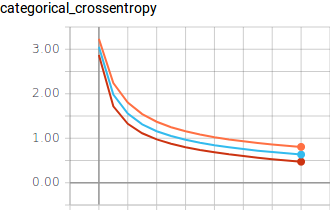
\includegraphics[width=0.5\linewidth]{part4/3CNN_train_category_crossentropy}}
	\end{minipage}
	\hfill
	\begin{minipage}[ht]{1\linewidth}
		\center{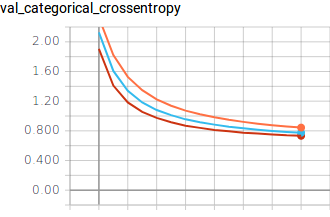
\includegraphics[width=0.5\linewidth]{part4/3CNN_val_category_crossentropy}}
	\end{minipage}
	\caption{Models train and validation category crossentropy by epochs}
	\label{img:3CNN_category_crossentropy}  
\end{figure}


\begin{table}[h]
	\centering
	\caption{Analysis of top k accuracy}
	\label{my-label}
	\begin{tabular}{| p{7cm} | p{3cm} | p{3cm} |}
		%	\begin{tabulary}{1.0\textwidth}{|L|L|L|L|L|L}
		\hline
		\textbf{Number of filters}  & \textbf{Train} & \textbf{Test}                                                    
		\\ \hline
		128   &  0.9259 & 0.9191
		\\ \hline
		256   &  0.9495 & 0.9286 
		\\ \hline
		512   &  0.9696 & 0.9342
		\\ \hline		
	\end{tabular}
\end{table}


According to the results, I can make assumption that models which have more filters show better accuracy. However, it is noticeable that model with 256 and 512 filters have quite different results on train and test sets (~3-5\% difference). It can be interpret as overfitting of these models. 


\begin{figure}[ht]
	\begin{minipage}[ht]{1\linewidth}
		\center{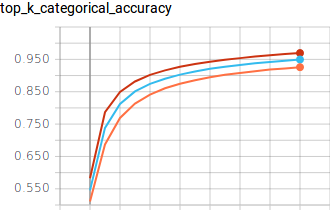
\includegraphics[width=0.5\linewidth]{part4/3CNN_train_top_k_accuracy}}
	\end{minipage}
	\hfill
	\begin{minipage}[ht]{1\linewidth}
		\center{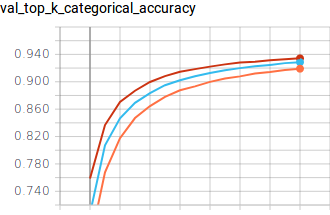
\includegraphics[width=0.5\linewidth]{part4/3CNN_val_top_k_accuracy}}
	\end{minipage}
	\caption{Models train and validation top k accuracy by epochs}
	\label{img:3CNN_top_k_accuracy}  
\end{figure}


\begin{figure}[ht] 
	\center
	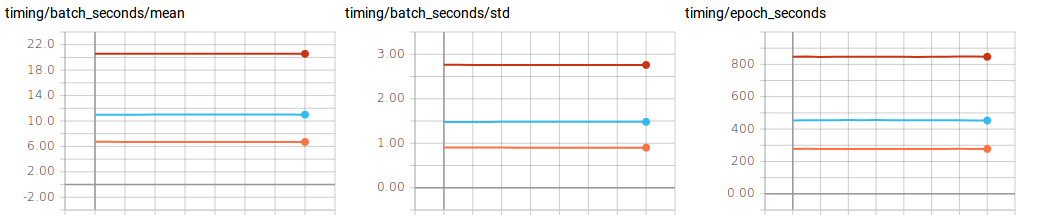
\includegraphics [scale=0.5] {part4/3CNN_timing}
	\caption{Models batch time by epochs} 
	\label{img:3CNN_timing}  
\end{figure}

\clearpage

Histograms of convolution layers looks almost the same. They do not change significantly from the initial distribution. That can mean they this layer do not learn much. 

\begin{figure}[ht]
	\begin{minipage}[ht]{1\linewidth}
		\center{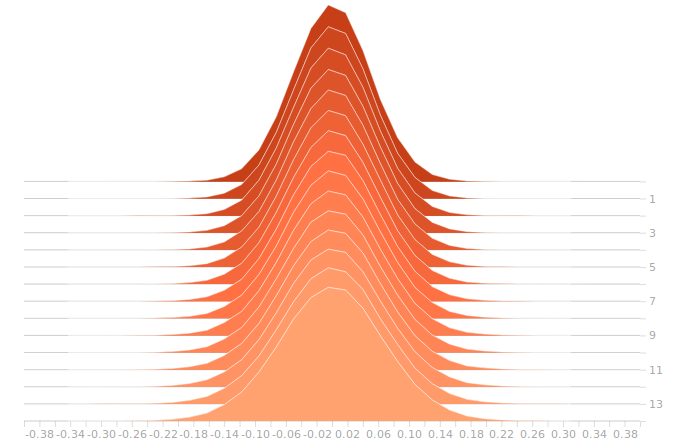
\includegraphics[width=0.5\linewidth]{part4/3CNN-conv-128.png} \\ а}
	\end{minipage}
	\hfill
	\begin{minipage}[ht]{1\linewidth}
		\center{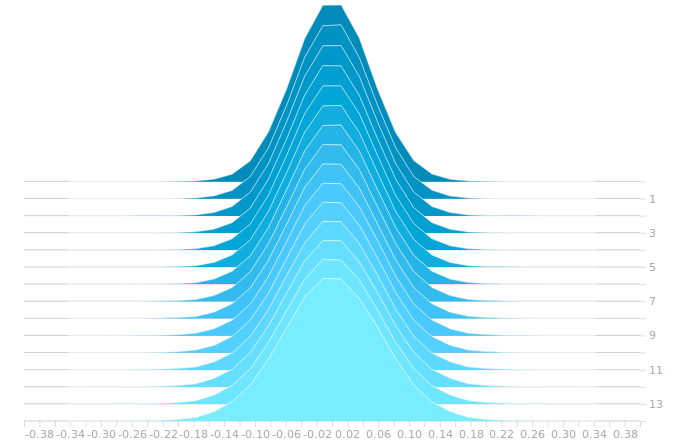
\includegraphics[width=0.5\linewidth]{part4/3CNN-conv-256.png} \\ b}
	\end{minipage}
	\begin{minipage}[ht]{1\linewidth}
		\center{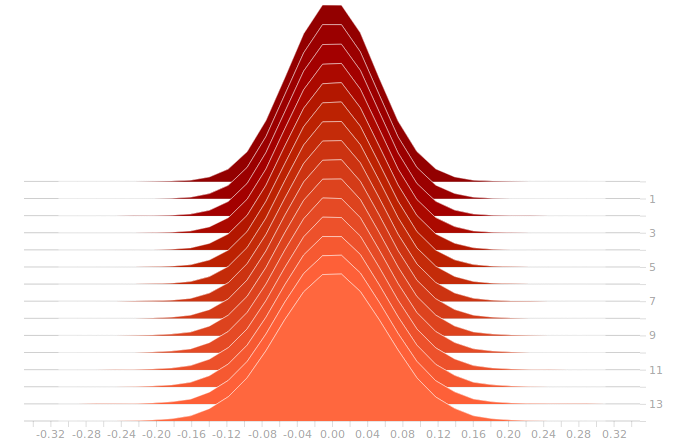
\includegraphics[width=0.5\linewidth]{part4/3CNN-conv-512.png} \\ c}
	\end{minipage}
	\caption{Convolutional model (a) 128;(b) 256; (c) 512 filters for each sizes [3, 4, 5]. Histogram of convolution layers}
	\label{img:3CNN_conv_layers}  
\end{figure}

\noindent
\\
\\
\\
\\
\\
Merged layers are also very similar, because of convolution layers.

\begin{figure}[ht]
	\begin{minipage}[ht]{1\linewidth}
		\center{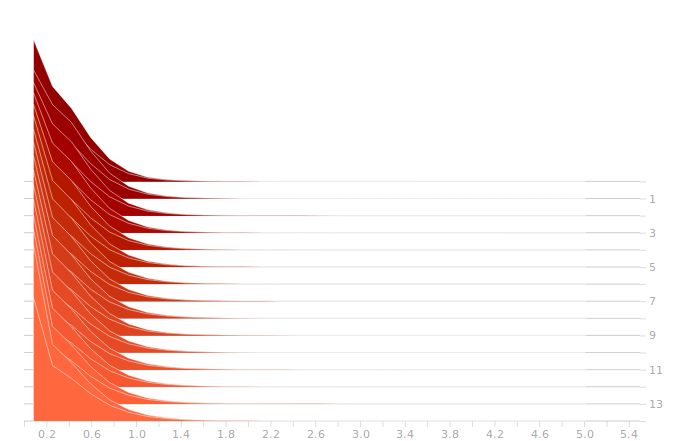
\includegraphics[width=0.45\linewidth]{part4/3CNN-merge3-128.png} \\ а}
	\end{minipage}
	\hfill
	\begin{minipage}[ht]{1\linewidth}
		\center{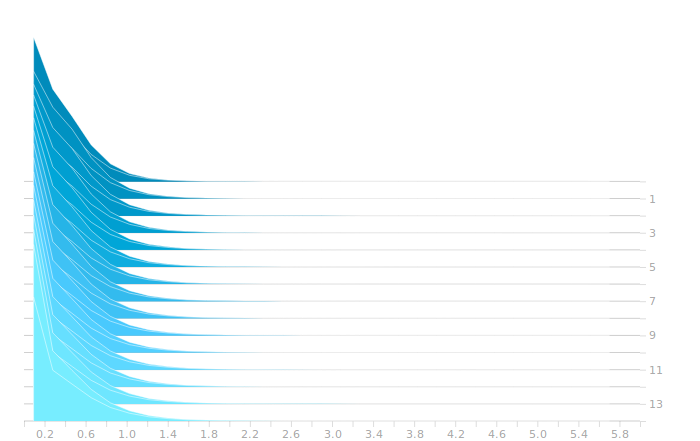
\includegraphics[width=0.45\linewidth]{part4/3CNN-merge3-256.png} \\ b}
	\end{minipage}
	\begin{minipage}[ht]{1\linewidth}
 		\center{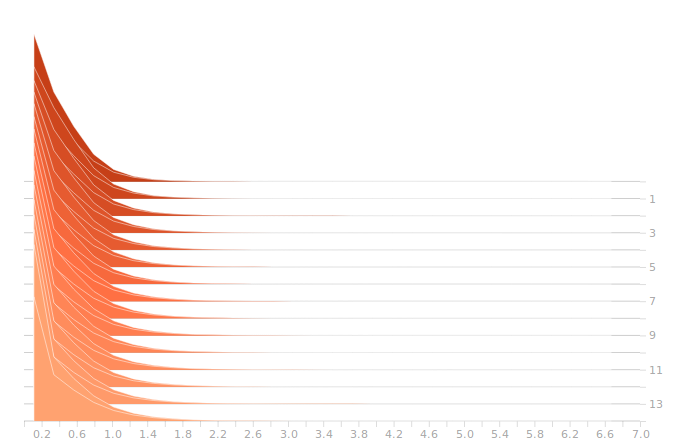
\includegraphics[width=0.45\linewidth]{part4/3CNN-merge3-512.png} \\ c}
	\end{minipage}
	\caption{Convolutional model (a) 128;(b) 256; (c) 512 filters for each sizes [3, 4, 5]. Histogram of merged layers}
	\label{img:3CNN_merged_layers}  
\end{figure}

\clearpage
The only difference we can see in dense layers. The model with 512 filters has normal distribution with lower variance comparing to the one with 128 filters. It is noticeable, that this the final distribution changed comparing to initial one, that means that layer learned some information. 

\begin{figure}[ht]
	\begin{minipage}[ht]{1\linewidth}
		\center{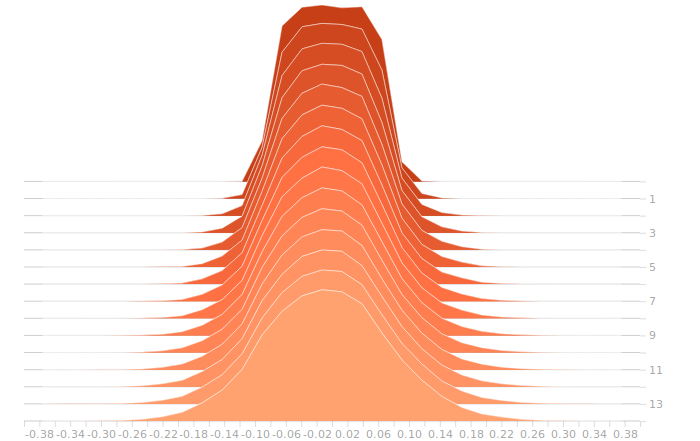
\includegraphics[width=0.5\linewidth]{part4/3CNN-dense-128.png} \\ а}
	\end{minipage}
	\hfill
	\begin{minipage}[ht]{1\linewidth}
		\center{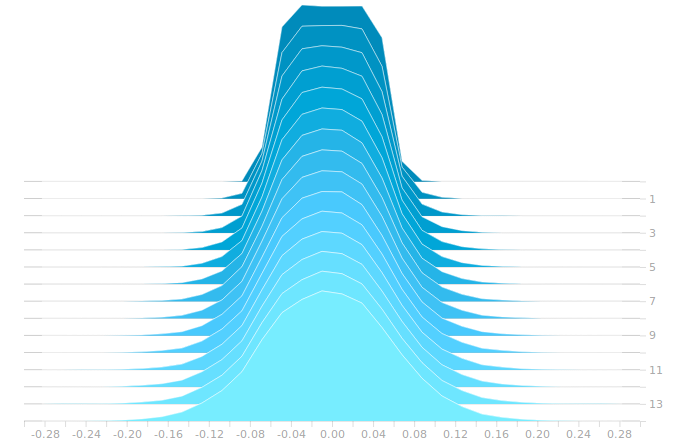
\includegraphics[width=0.5\linewidth]{part4/3CNN-dense-256.png} \\ b}
	\end{minipage}
	\begin{minipage}[ht]{1\linewidth}
		\center{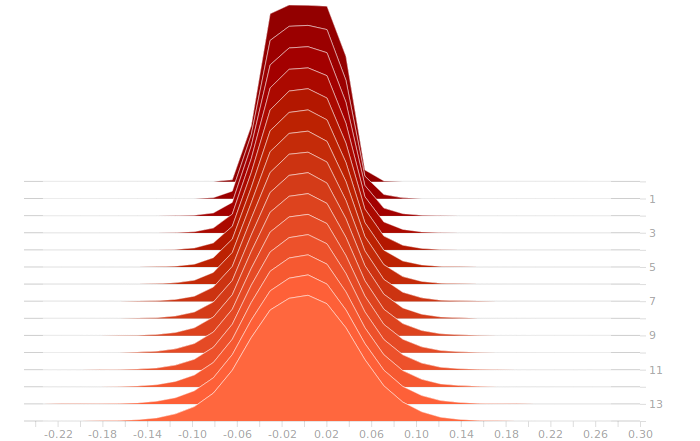
\includegraphics[width=0.5\linewidth]{part4/3CNN-dense-512.png} \\ c}
	\end{minipage}
	\caption{Convolutional model (a) 128;(b) 256; (c) 512 filters for each sizes [3, 4, 5]. Histogram of dense layers}
	\label{img:3CNN_dense_layers}  
\end{figure}

\clearpage
The CNN model requires less resources for training than bi-LSTM. Therefore, I was able to use 
5 times bigger batch size. We can see consumption of resources in the Figure \ref{img:resources_CNN}

\begin{figure}[ht] 
	\center
	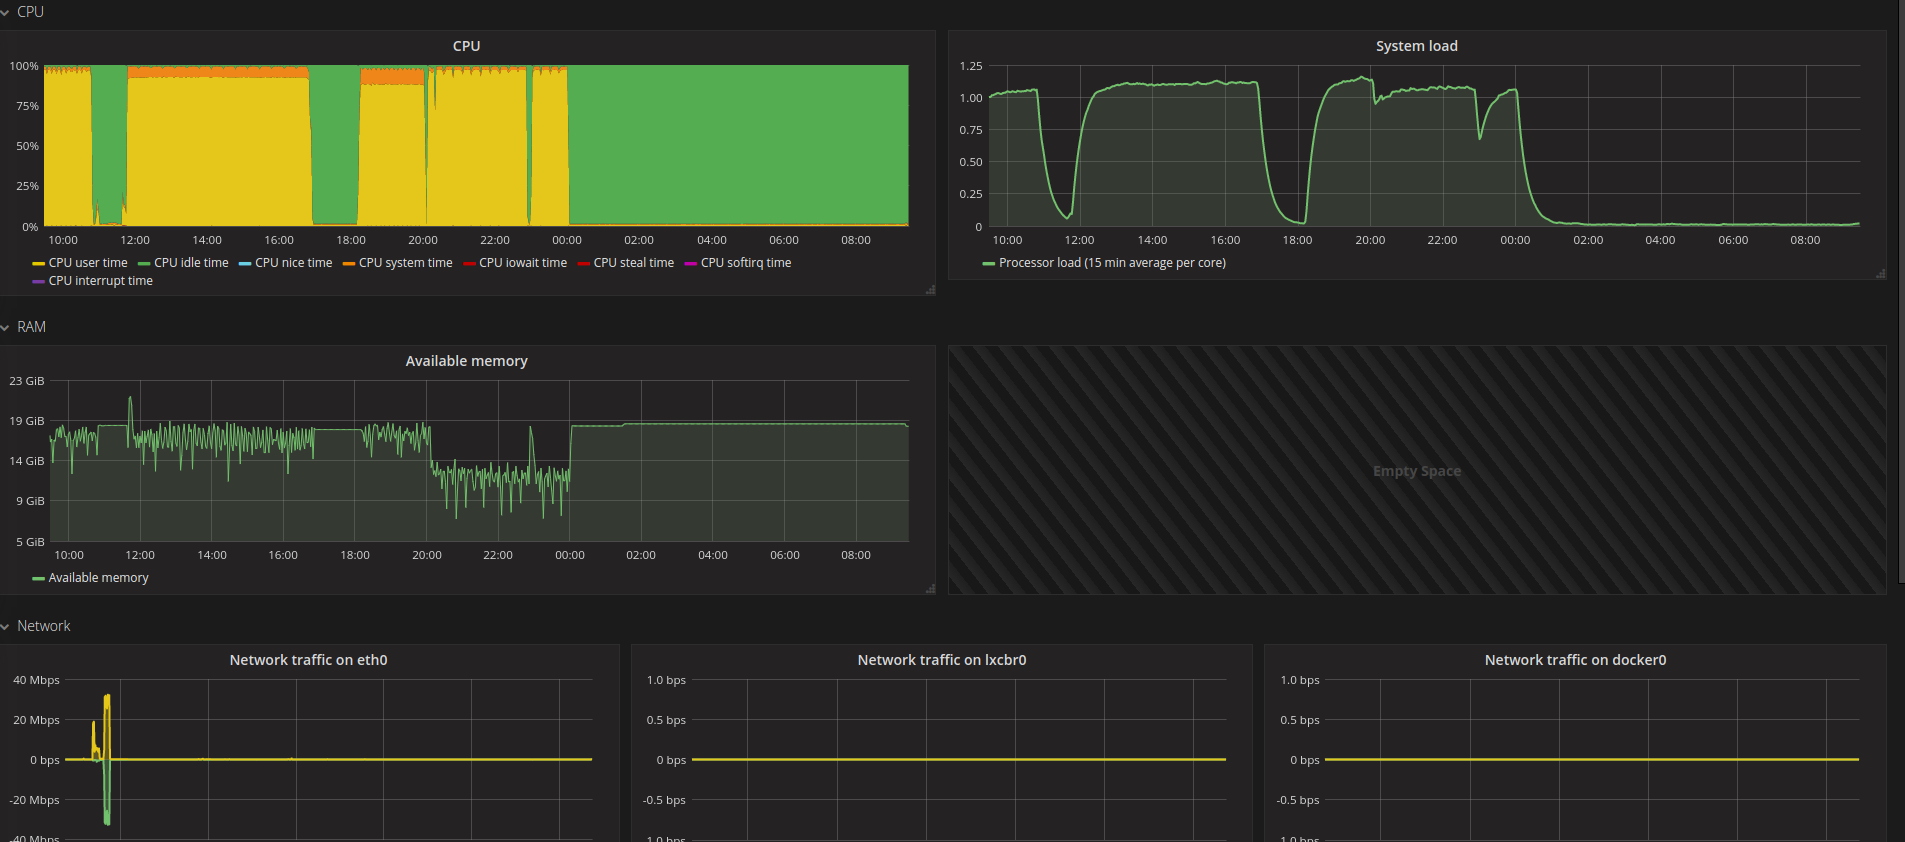
\includegraphics [scale=0.2] {part4/resources_CNN}
	\caption{CPU resources which were used while training CNN.} 
	\label{img:resources_CNN}  
\end{figure}




\clearpage
\section{Convolution neural network with different regularization} \label{sect4_4}

In this section I tried to use different regularization to get rid of overfitting. I test all these approaches on the CNN with 512 filters. I made following changes in the initial architecture of the model:

%blue-modified_epoch15_outdim183_nbfilters512_drop10.5_drop20.2
%grey-withl2regul_0.001_0.01_adam_epoch15_outdim183_nbfilters512_drop10.25_drop20.25
%pink-withl2regul_0.001_0.01_epoch15_outdim183_nbfilters512_drop10.25_drop20.25
%cyan-withl2regul_epoch15_outdim183_nbfilters512_drop10.25_drop20.25

\begin{enumerate}
	\item I we saw in the previous section the convolution layer did not train enough so I thought it was caused because of big dropout rate. Therefore I decreased it in two times.
	\item I also added the l2-regularization equals to 0.001 for convolution layers and changed dropout rate to 0.25 both for dense and convolution layers. Moreover, I decided to configure my training algorithm, so I used Adam with learning rate 1e-4. 
	\item The same configuration as previous but Adam was with learning rate 1e-3.
	\item The same as 2, but l2-regularization was equal to 0.01
\end{enumerate}

\begin{table}[h]
	\centering
	\caption{Analysis of top k accuracy}
	\label{my-label}
	\begin{tabular}{| p{7cm} | p{3cm} | p{3cm} |}
		%	\begin{tabulary}{1.0\textwidth}{|L|L|L|L|L|L}
		\hline
		\textbf{Number of filters}  & \textbf{Train} & \textbf{Test}                                                    
		\\ \hline
		128   &  0.9259 & 0.9191
		\\ \hline
		256   &  0.9495 & 0.9286 
		\\ \hline
		512   &  0.9696 & 0.9342
		\\ \hline		
	\end{tabular}
\end{table}

\begin{table}[h]
	\centering
	\caption{Analysis of top k accuracy}
	\label{my-label}
	\begin{tabular}{| p{7cm} | p{3cm} | p{3cm} |}
		%	\begin{tabulary}{1.0\textwidth}{|L|L|L|L|L|L}
		\hline
		\textbf{Number of filters}  & \textbf{Train} & \textbf{Test}                                                    
		\\ \hline
		128   &  0.9259 & 0.9191
		\\ \hline
		256   &  0.9495 & 0.9286 
		\\ \hline
		512   &  0.9696 & 0.9342
		\\ \hline		
	\end{tabular}
\end{table}

\begin{table}[h]
	\centering
	\caption{Analysis of top k accuracy}
	\label{my-label}
	\begin{tabular}{| p{7cm} | p{3cm} | p{3cm} |}
		%	\begin{tabulary}{1.0\textwidth}{|L|L|L|L|L|L}
		\hline
		\textbf{Number of filters}  & \textbf{Train} & \textbf{Test}                                                    
		\\ \hline
		128   &  0.9259 & 0.9191
		\\ \hline
		256   &  0.9495 & 0.9286 
		\\ \hline
		512   &  0.9696 & 0.9342
		\\ \hline		
	\end{tabular}
\end{table}

\begin{figure}[ht]
	\begin{minipage}[ht]{1\linewidth}
		\center{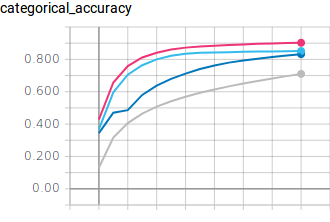
\includegraphics[width=0.5\linewidth]{part4/4CNN_train_category_accuracy}}
	\end{minipage}
	\hfill
	\begin{minipage}[ht]{1\linewidth}
		\center{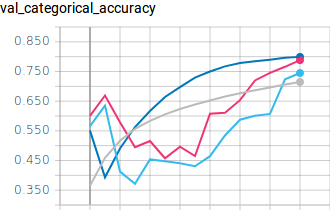
\includegraphics[width=0.5\linewidth]{part4/4CNN_val_category_accuracy}}
	\end{minipage}
	\caption{Models train and validation categorical accuracy by epochs}
	\label{img:4CNN_categorical_accuracy}  
\end{figure}


\begin{figure}[ht]
	\begin{minipage}[ht]{1\linewidth}
		\center{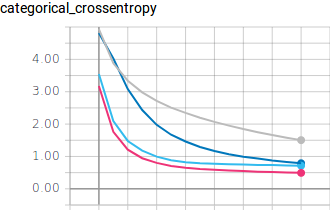
\includegraphics[width=0.5\linewidth]{part4/4CNN_train_category_crossentropy}}
	\end{minipage}
	\hfill
	\begin{minipage}[ht]{1\linewidth}
		\center{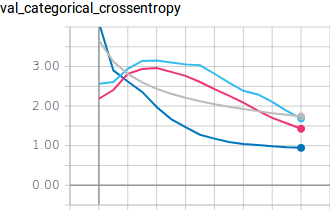
\includegraphics[width=0.5\linewidth]{part4/4CNN_val_category_crossentropy}}
	\end{minipage}
	\caption{Models train and validation category crossentropy by epochs}
	\label{img:4CNN_category_crossentropy}  
\end{figure}

\begin{figure}[ht]
	\begin{minipage}[ht]{1\linewidth}
		\center{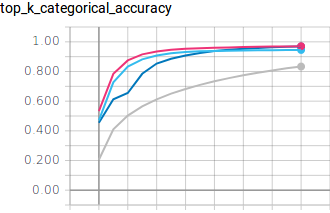
\includegraphics[width=0.5\linewidth]{part4/4CNN_train_top_k_accuracy}}
	\end{minipage}
	\hfill
	\begin{minipage}[ht]{1\linewidth}
		\center{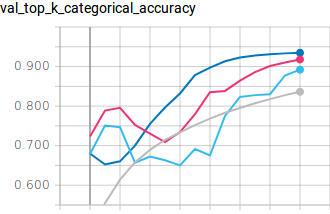
\includegraphics[width=0.5\linewidth]{part4/4CNN_val_top_k_accuracy}}
	\end{minipage}
	\caption{Models train and validation top k accuracy by epochs}
	\label{img:4CNN_top_k_accuracy}  
\end{figure}

\begin{figure}[ht] 
	\center
	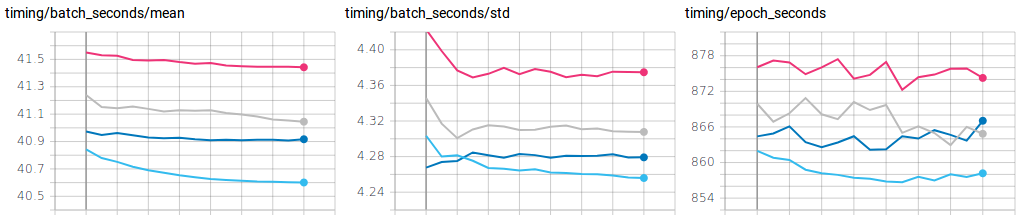
\includegraphics [scale=0.5] {part4/4CNN_timing}
	\caption{Models batch time by epochs} 
	\label{img:4CNN_timing}  
\end{figure}



\begin{figure}[ht]
	\begin{minipage}[ht]{1\linewidth}
		\center{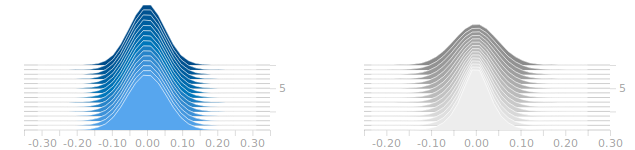
\includegraphics[width=0.5\linewidth]{part4/4CNN-conv-1.png} \\ а}
	\end{minipage}
	\hfill
	\begin{minipage}[ht]{1\linewidth}
		\center{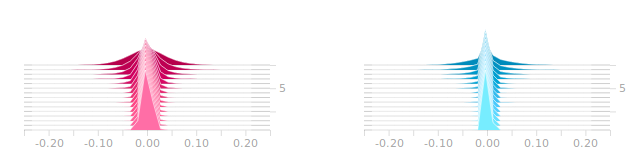
\includegraphics[width=0.5\linewidth]{part4/4CNN-conv-2.png} \\ b}
	\end{minipage}
	\caption{Convolutional model (a) 128;(b) 256; (c) 512 filters for each sizes [3, 4, 5]. Histogram of convolution layers}
	\label{img:category_crossentropy}  
\end{figure}


\begin{figure}[ht]
	\begin{minipage}[ht]{1\linewidth}
		\center{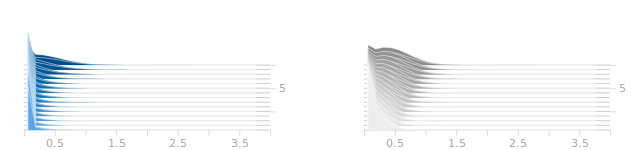
\includegraphics[width=0.5\linewidth]{part4/4CNN-merge3-1.png} \\ а}
	\end{minipage}
	\hfill
	\begin{minipage}[ht]{1\linewidth}
		\center{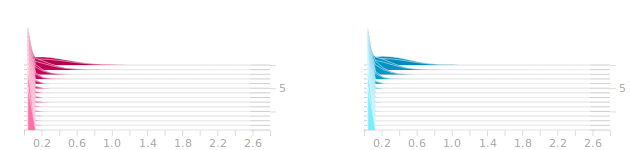
\includegraphics[width=0.5\linewidth]{part4/4CNN-merge3-2.png} \\ b}
	\end{minipage}
	\caption{Convolutional model (a) 128;(b) 256; (c) 512 filters for each sizes [3, 4, 5]. Histogram of convolution layers}
	\label{img:category_crossentropy}  
\end{figure}


\begin{figure}[ht]
	\begin{minipage}[ht]{1\linewidth}
		\center{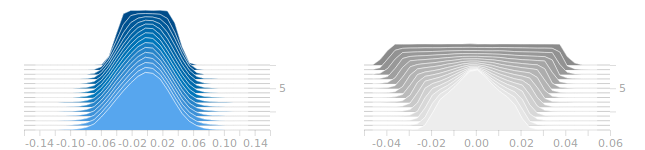
\includegraphics[width=0.5\linewidth]{part4/4CNN-dense-1.png} \\ а}
	\end{minipage}
	\hfill
	\begin{minipage}[ht]{1\linewidth}
		\center{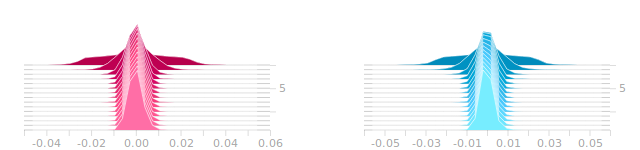
\includegraphics[width=0.5\linewidth]{part4/4CNN-dense-2.png} \\ b}
	\end{minipage}
	\caption{Convolutional model (a) 128;(b) 256; (c) 512 filters for each sizes [3, 4, 5]. Histogram of convolution layers}
	\label{img:category_crossentropy}  
\end{figure}

\clearpage
\section{Final model} \label{sect4_5}

\clearpage
\section{Classification results} \label{sect4_6}



